\section{Introduction}

The field of image and video synthesis is large and continuously expanding. While image generation has come a long way, recent advancements in video synthesis emerged recently, highlighted by the significant breakthrough of OpenAI's Sora model \cite{sora_website}. A solid foundation in image synthesis techniques is essential to fully comprehend the methodologies and techniques involved in video synthesis.

In this work we will review two main models that are used as a basis in image and video generation models: Generative Adversarial Networks (GANs) \cite{gan} \ref{sec:gan}, and Diffusion Probabilistic Models (DPMs) \cite{diffusion_models} \cite{ddpm}, \ref{sec:ddpm}.

In generative models we are given a set of data points (e.g. images) and our goal is to create a new sample (new image) from this dataset. That is, we don't want to randomly select an image from the dataset, but rather we want to create a new image that does not appear in the dataset, but is similar to it. The key word is "similar" - mathematically speaking, we are talking about predicting the probability function of the dataset. That is, the model needs to learn the underlying distribution of the dataset and create new samples that represent the same distribution. Generative models provide an efficient method for analyzing and understanding unlabeled data in unsupervised learning.

Advanced image synthesis models like DALL-E \cite{dalle} and Stable Diffusion \cite{stable_diffusion} represent a significant milestone in the field. While recent models may not offer groundbreaking advancements, the landscape of long video synthesis remains relatively unexplored. Video synthesis presents unique challenges compared to image synthesis, primarily due to the introduction of the temporal dimension.

New models for generating images and videos are developed by building upon existing models, enhancing them through innovative techniques and adjustments. In this work we explore the VQ-GAN model \cite{vqgan} \ref{vqgan} which combines the GAN model \cite{gan} \ref{sec:gan} with the VQ-VAE model \cite{vqvae} \ref{vqvae} and the Transformer model \cite{transformer} (appendix \ref{appendix:transformers}) together. Notably, VQ-GAN generates images based on textual descriptions, converting text inputs into visual outputs that reflect the text's description. The VQ-VAE model, derived from the VAE model \cite{vae} \ref{sec:vae} and employing vector quantization technique \cite{vqvae} \ref{vq}, is itself an advancement of the Autoencoder model \cite{autoencoder} \ref{sec:vae}. In short, understanding these models and their inner workings requires prior familiarity with their foundations and previous works.

Another example is the Variational Autoencoder (VAE) \cite{vae} \ref{sec:vae} model, which is used as a basis in VQ-VAE model. 

\begin{figure}
    \centering
    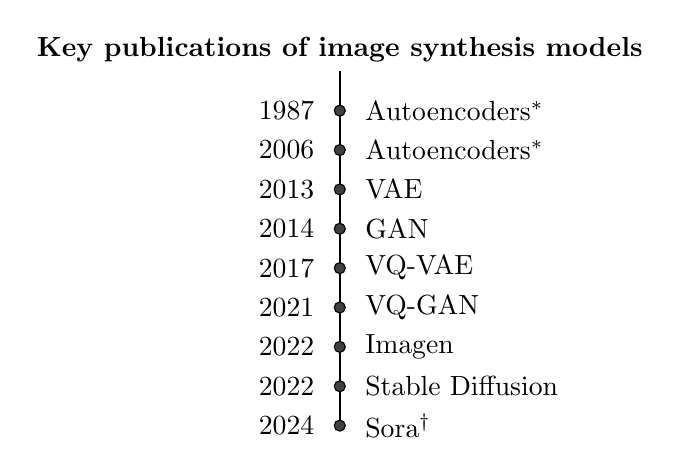
\begin{tikzpicture}
        \def\step{0.5} % step size for vertical spacing
        \def\numtimeline{9} % Number of events in the timeline

        % Define timeline line
        \draw[thick, color=black] (0,0) -- (0,-\numtimeline*\step);

        % Define timeline events with adjusted positions
        \foreach \i/\year/\text in 
        {
            1/1987/Autoencoders$^*$, 
            2/2006/Autoencoders$^*$, 
            3/2013/VAE, 
            4/2014/GAN, 
            5/2017/VQ-VAE,
            6/2021/VQ-GAN,
            7/2022/Imagen,
            8/2022/Stable Diffusion,
            9/2024/Sora$^\dag$
        } {
        \draw[fill=darkgray] (0,-\i*\step) circle (2pt);
        \node[anchor=east] at (-0.2,-\i*\step) {\year};
        \node[anchor=west] at (0.2,-\i*\step) {\text};
        }

        % Define timeline title
        \node[anchor=south] at (0,0) {\textbf{Key publications of image synthesis models}};
    \end{tikzpicture}
    \caption{Chronology of key image generation models publications $^*$The earliest mention of autoencoders appears in an 1986 publication \cite{autoencoder_original_paper_1986}, however the model was not widely used until 2006 when Hinton published a paper that uses autoencoders for dimensionality reduction \cite{autoencoder_2006_paper} which sparked interest in the model again.$^\dag$Although Sora \cite{sora_website} is not specifically an image generation model, its considered a significant advancement in video synthesis field, which largely relies on image generation.}
    \label{fig:timeline}
  \end{figure}

\subsection{Mathematical Formulation of Generative Models}
Mathematically speaking, let $x$ be a random variable representing a single data point (e.g. an image) of a dataset ${x_1,x_2,...,x_n}$. And let $p(x)$ denote the true probability density function (PDF) of the dataset, then our objective (as in generative modeling) is to learn a function $q(x;\theta)$ that approximates the true data distribution $p(x)$ (where $\theta$ is the model's parameters). The goal is to estimate $p(x)$ such that new samples $\hat{x} \in p(x)$ drawn from this distribution resemble the dataset.

Most of the time, it is infeasible to calculate directly $p(x)$ because computing the exact probability density for high-dimensional data is computationally expensive and often requires integrating over a large number of variables. This complexity leads to intractable calculations, making it difficult to directly model $p(x)$. Instead, we use various techniques to approximate it, and we denote it as: $q(x;\theta) \sim p(x)$.

\subsection{Approximating the Data Distribution}

In order to approximate $p(x)$ we can use a generative model, where the training objective is to learn the parameters $\theta$ of the model. The success or failure of the model to correctly approximate the dataset distribution can be evaluated using different loss functions, such as maximizing likelihood functions (Appendix \ref{appendix:likelihood_function}), minimizing Kullback-Leibler (KL) divergence, or using adversarial training loss (in the case of GANs).

\subsection{Sampling}

Once trained, the generative model can be used to generate new samples $\hat{x} \sim q(x;\theta)$. Sampling data point $\hat{x}$ will be consistent with the patterns and characteristics of the original dataset, as the model has learned to approximate the true data distribution. Each model will have different strategies to sample. For example, in GANs a random noise vector is sampled from a normal distribution and passed through the generator to generate a new sample, and in VQ-GAN a transformer is used to generate latent codes that are then passed through the decoder to generate an image.

\subsection{Evaluation metrics}

Evaluation of the trained model is done using metrics such as sample quality, diversity (variety in generated samples), and coverage (how well the model covers the data distribution). As we will find later, one of the main problems of the GAN model is called 'mode collapse' \ref{gan_mode_collapse} which causes instability of the model during training, which is manifested in large fluctuations in the loss function or in the fact that the generator fails to converge to an optimal solution that represents the entire distribution of training data. In other words, the model's output isn't diverse enough and only focuses on specific modes of the data distribution (e.g. generating only one type of image, like a cat, whereas the dataset is a collection of all animals).





\textbf{Inception Score.} One of the most common metrics used to evaluate the quality of generated samples is the Inception Score (IS) \cite{is_score}. The IS metric measures the quality and diversity of the generated samples. A good generative model should not only produce images that look visually realistic but also capture the underlying statistical properties of the dataset. A high IS score indicates that the generated samples are both realistic and diverse. IS uses pre-trained Inception V3 model \cite{inception_v3_model} to extract features and classify images to labels. The Inception V3 model is made of multiple convolutional layers and pooling layers and the last layers are fully connected layers with softmax activation function (output is probability of labels) that output the class labels (1000 classes). Two generative models are compared to each other with IS by running the same Inception V3 model, and comparing their scores relatively. The IS is calculated by first computing the conditional entropy of the generated samples given the class label: 

\[
    p(y) = \frac{1}{N} \sum_{i=1}^{N} p(y|x_i)
\] 

(where $y$ is the class label and $x$ is an image, $p(y|x)$ is the conditional probability of the label $y$ given image $x$) (i.e., the diversity of generated samples) and then computing the \textbf{KL divergence} between the marginal distribution of the generated samples and the conditional distribution:

\[
    D_{\text{KL}}(p(y|x) \| p(y)) = \sum_{y} p(y|x) \log \frac{p(y|x)}{p(y)}
\]

(where $p(y)$ is the marginal probability of the label across the set of generated images, and $D_{KL}$ is the Kullback-Leibler (KL) divergence between the conditional label distribution $p(y|x)$ and marginal label distribution $p(y)$). Finally, we get the IS score as:

\[
    \text{IS} = \exp \left( \frac{1}{N} \sum_{i=1}^{N} D_{\text{KL}}(p(y|x_i) \| p(y)) \right) = \exp(\mathbb{E}_{x \sim p_g} \left[ D_{\text{KL}} \left( p(y | x) \Vert p(y) \right) \right])
\]

Where $p_g$ is the distribution of the generated images. The IS score is the exponential of the sum of these two terms. A high IS score indicates that the generated samples are both realistic and diverse because $p(y|x)$ should be sharp (i.e. indicating generated samples are high quality), and $p(y)$ should be uniform (i.e. generated samples are diverse).






\textbf{FID Score.} Frechet Inception Distance (FID) score \cite{fid_score} is an improvement on the Inception Score and is more recent. The FID score also measures the similarity between the generated samples and the real data distribution, and the diversity. FID aims to capture this by comparing the feature distributions, not just individual image similarity. The lower the FID score, the better the model is at generating samples that resemble the real data distribution. FID leverages a pre-trained image classification model (which is also typically Inception V3 model), to extract high-level features from both the generated images and the dataset. These features capture the essential characteristics of the images, like shapes, textures, and object relationships. Then, it is possible to compare generative models based on the similarity of these features relatively to the same dataset, compared to just looking at the labels in Inception Score. The FID score is calculated as:

\begin{equation}
    \text{FID} = ||\mu_x - \mu_g||^2 + Tr(\Sigma_x + \Sigma_g - 2(\Sigma_x\Sigma_g)^{1/2})
    \label{eq:fid_score}
\end{equation}

where $\mu_x$ and $\Sigma_x$ are the mean and covariance of the feature distribution of the dataset, and $\mu_g$ and $\Sigma_g$ are the mean and covariance of the feature distribution of the generated images. The FID score is the Euclidean distance between the means and the trace (matrix operation) of the covariance matrices. A lower FID score indicates that the generated samples are more similar to the real data distribution.

